%!Mode:: "TeX:UTF-8"
%!TEX program = xelatex
%!TEX TS-program = xelatex
%!TEX encoding = UTF-8 Unicode
%
% Author: Rickjin (ZhihuiJin@gmail.com)
% Author: Leijun  (leijun00@gmail.com)

\chapter{永远的倒霉蛋}

运气是人生哲学里非常重要的一个话题,我们常听说:人生除了勤奋努力,还是需要一点
运气的。就连比尔盖茨也把他的成功归结为运气。不过心理学的研究表明:人们对运气的
看法是非常奇特的,绝大多数的人都认为别人瓜地里的瓜比自己地里的瓜甜,别人的老婆
比自己的漂亮,别人的运气要远比自己好,而自己永远是那个倒霉蛋。如果从数学上来研
究运气的话,它是和概率论紧密相关的。如果大家具备一点概率知识的话,应该会发现自
然常数 $e$ 和概率紧密相关,经常出现在概率论里面,所以 $e$ 和运气也紧密相关。我
们从一个倒霉蛋 Cassie 的故事说起。

\section{年会抽奖}

有过工作经验的人都知道每年天上都会掉下来几个馅饼,但是能不能被砸中就很难说了。
公司年会通常会设置特等奖、一等奖、二等奖和三等奖等奖项,奖品也非常丰厚,有 
iPad、iPhone 等,房地产公司的奖品甚至是豪车(宝马、奔驰等)和豪宅。每个人都非常
期待自己能中奖,但绝大多数人最后都是扫兴而归,故事的主人公 Cassie 就是这样一位
普通的企业职工。

Cassie 的第一份工作在一家小公司,公司只有十个员工,公司年会的时候,老板准备了十
份礼物,抽了十次奖,可是 Cassie 的运气不好,一次都没中,她非常沮丧。可是 Cassie
转念一想,十次抽奖,一次都不中的概率应该也不低,所以她也没有太介意。第二年,
Cassie 跳槽到一家有一万员工的大公司,很幸运遇到了一个土豪老板。
\begin{figure}[H]
\centering

\includegraphics[scale=0.4]{lottery/boss.png}
\caption{土豪老板}
\centering
\end{figure}

土豪老板在公司的年会上宣布:今年的抽奖人人有份,公司准备了一万份奖品,抽一万次
奖。每个人听到这个消息都非常兴奋,天上掉下来一万个馅饼,不被砸中实在是天理难容
,说不过去。Cassie 非常期待自己能中奖,可以结果完全出乎意料之外,一万个馅饼一个
都没砸中 Cassie。更悲惨的是,隔壁的帅哥居然连中十个。Cassie 觉得自己的人生太悲
催了,最倒霉的事情就是自己倒霉的时候看到旁边的帅哥那么幸福。
\begin{figure}[H]
\centering
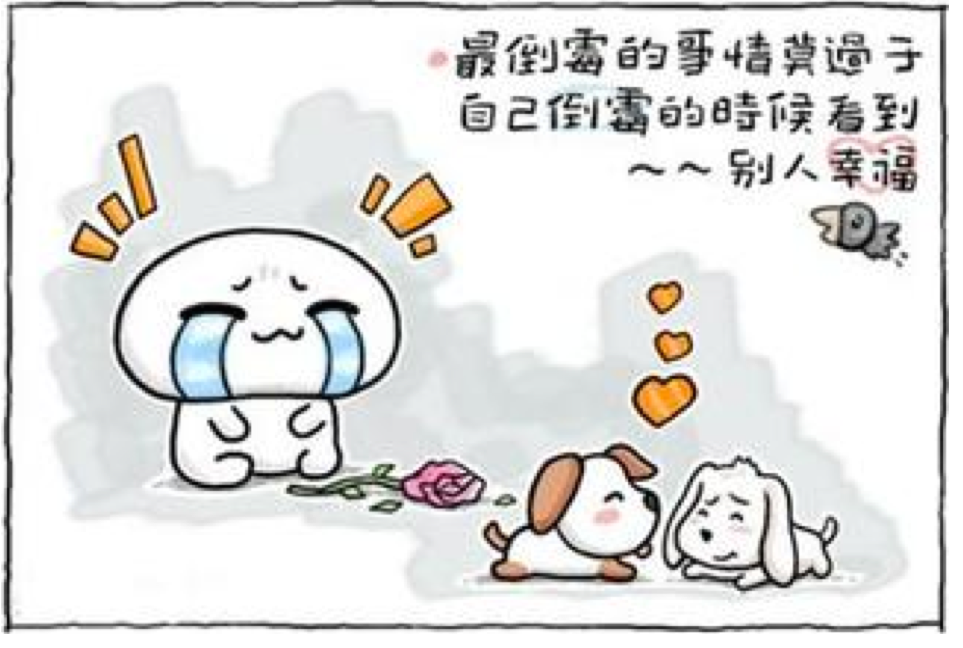
\includegraphics[scale=0.6]{lottery/badluck.png}
\caption{倒霉时刻}
\centering
\end{figure}

Cassie 怎么也想不明白,去年十次抽奖一次没中还可以理解,今年是一万次抽奖,自己能
中一次的概率应该很高,怎么就恁是没中呢?她觉得自己的人生一定是被诅咒了,开始怀
疑自己的人生。
\begin{figure}[H]
\centering
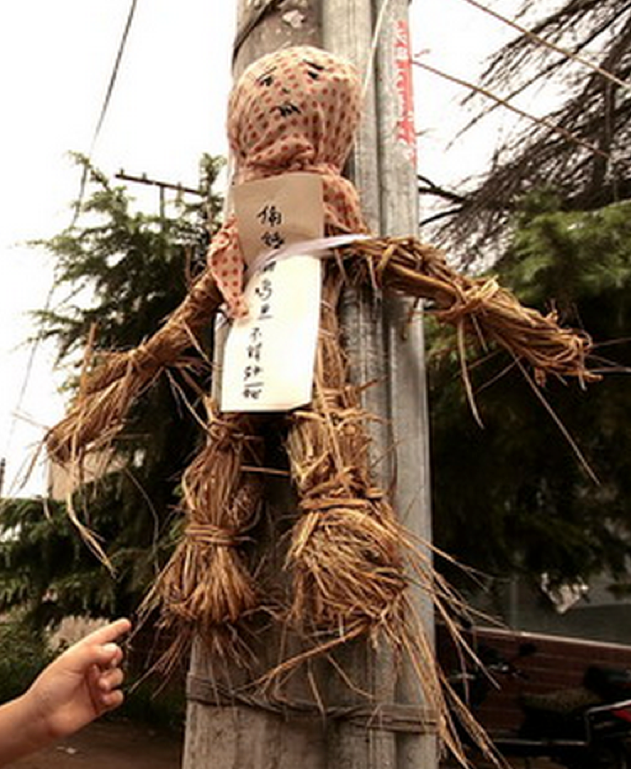
\includegraphics[scale=0.5]{lottery/curse.png}
\caption{诅咒的人生}
\centering
\end{figure}

我们从数学的角度帮 Cassie 分析一下她在两次公司年会中中奖的概率到
底有多高。假设公司有 $n$ 个人,一次抽奖每个人中奖的概率都是 $1/n$,不中奖的概
率是 $1-1/n$,每次抽奖都是一个独立事件,根据乘法原理 $n$ 次不中奖的概率为:
 $$ p_n = (1- \frac1n)^n $$
Cassie 的第一个公司 $n=10$,直觉上这个不中奖概率还挺高。第二个公司$ n=10000$,
不中奖概率是一个小于 1 的数的 10000 次方,直觉上应该很小很小。网络上流传着这样
两个经典等式:
$$ 1.01^{365} = 37.8 $$
$$ 0.99^{365} = 0.03 $$
只要每天增加一点正能量,一年后的正能量就会变成 37.8 倍,只要每天增加一点负能量,
一年后基本就不剩正能量了。那么一个 小于 1 的数的 10000 次方到底是多少呢?我们帮
 Cassie 算一下,整理成表格。
\begin{table}[htbp]
\centering
\caption{不中奖概率}
\begin{tabular}{|l|l|l|}
\hline
     n     & $ p_n $ & $ 1/p_n $ \\ \hline
     10    & 0.349   & 2.865     \\ \hline
     100   & 0.366   & 2.732     \\ \hline
     1000  & 0.368   & 2.717     \\ \hline
     10000 & 0.368   & 2.717     \\ \hline
\end{tabular}
\end{table}

我们发现,$n$ 取 10,100,1000, 10000 的时候,不中奖的概率并没有太大的区别,
随着 $n$ 的增大,不中奖的概率甚至收敛到一个固定的值,这个数并不是一个很小的数,
有点违背我们的直觉。我们稍微做一下变换,把这个概率求倒数,会发现这个倒数最后
收敛到 2.717 ,这不就是我们的自然常数 $e$ 吗?$e$ 再一次出现在我们的日常生活中!

\section{不走运是常态}

实际在数学上存在这样一个式子:
$$ \lim_{n \rightarrow +\infty } (1 - \frac1n)^n = \frac1e $$

\begin{figure}[htbp]
\centering
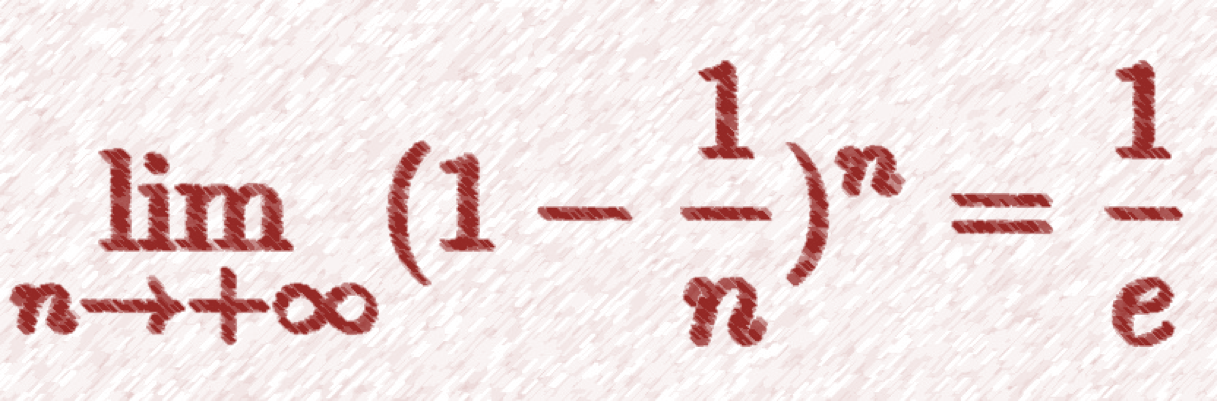
\includegraphics[width=0.6\textwidth]{lottery/e.png}
\caption{中奖概率}
\centering
\end{figure}

证明过程也不难:
\begin{align*}
\lim_{n \rightarrow +\infty } (1 - \frac1n)^n & = \lim_{n \rightarrow +\infty } (\frac {n-1} {n})^n   \\
&=  \frac {1} {\displaystyle \lim_{n \rightarrow +\infty } (\frac {n} {n-1})^n} \\
&=  \frac {1} {\displaystyle \lim_{n \rightarrow +\infty } ( 1 + \frac {1}{n-1})^n}  \\
&=  \frac {1} {\displaystyle \lim_{n \rightarrow +\infty } ( 1 + \frac {1}{n-1})^{n-1} (1+\frac {1} {n-1})} \\
&=  \frac {1} {e \displaystyle \lim_{n \rightarrow +\infty } (1+\frac {1} {n-1})} \\
&= \frac1e
\end{align*}

不管是 10 个人,还是 10000 个人,其实不中奖的概率是非常稳定的,接近 0.368。
不走运其实是人生常态,不用太介意,37\% 的不中奖概率其实很高了,不中奖其实是
一个大概率事件。

实际在概率上有大量的例子都是和人的直觉违背的,按数学家的话说,就是人的脑子里缺
一根弦,没有一个理解概率计算的好的机制。概率对理解人生中的运气非常有帮助,在人
生哲学中扮演着相当重要的角色。互联网上有一些数学的禅师给了我们一些教诲:数学学
得好将来一定比别人幸福,数学学得好的人一定不会想不开,那些跳楼的都是文科生。
